% !TeX root = ../paper.tex
\subsection{Model Building and Training}
\label{sec:model-building}

We implemented and evaluated three distinct approaches: \ac{RAG}, model
fine-tuning, and a hybrid combination. This section details the architecture, training pipeline, and technical implementation of each method

\subsubsection{\ac{RAG}}
\label{sec:rag-pipeline}

\paragraph{Architecture Overview}

\ac{RAG} is essential in medical applications because it enables dynamic updates to medical knowledge bases without requiring model retraining, which is particularly important given the continuously evolving nature of medical information. \ac{RAG} systems, including LightRAG, can ingest diverse medical data sources such as textbooks, case reports, and fact sheets, and store them in a database. When a query is given, the system retrieves relevant information from the knowledge base.

Unlike conventional RAG pipelines that primarily rely on vector similarity search, LightRAG has a graph-based approach. In LightRAG, entities represent meaningful medical concepts (e.g., diseases, symptoms, or drugs), while relationships capture the semantic connections between these entities (e.g., causes, treats, or associated with). By extracting entities and their relationships, LightRAG is able to retrieve more relevant information and uncover deeper contextual connections within the data.

\paragraph{RAG Implementation Pipeline}

In a general RAG system, there are three distinct phases that define its operation: the data ingestion phase, the retrieval phase, and the generation phase. However, in our system, along side with LightRAG, we already have an \ac{MLLM} model available and want to retain control over context engineering. Therefore, in this work, we omit the final generation phase of LightRAG and focus solely on the first two phases.

\begin{enumerate}[label=\roman*.]
    \item Data ingestion phase: As illustrated in Fig.~\ref{fig:data-ingestion}, uploaded data sources are first processed according to their modality, specifically separating text and image inputs. Text-only documents are supported by default and therefore require no additional preprocessing. For images, we use an adapter from GraphRAG pipeline to generate textual descriptions that map each image to a corresponding text representation. All textual content is then aggregated and segmented into appropriately sized chunks. For each data chunk, an \ac{LLM} is invoked to extract entities and relationships and the knowledge graph is gradually formulated. The extracted entities and relationships are subsequently deduplicated to eliminate redundancy and stored in two databases: a vector database that holds embedded metadata, and a key–value database that holds the mappings among entities, relationships, and data chunks.
    \begin{figure}[htbp]
    \centering
    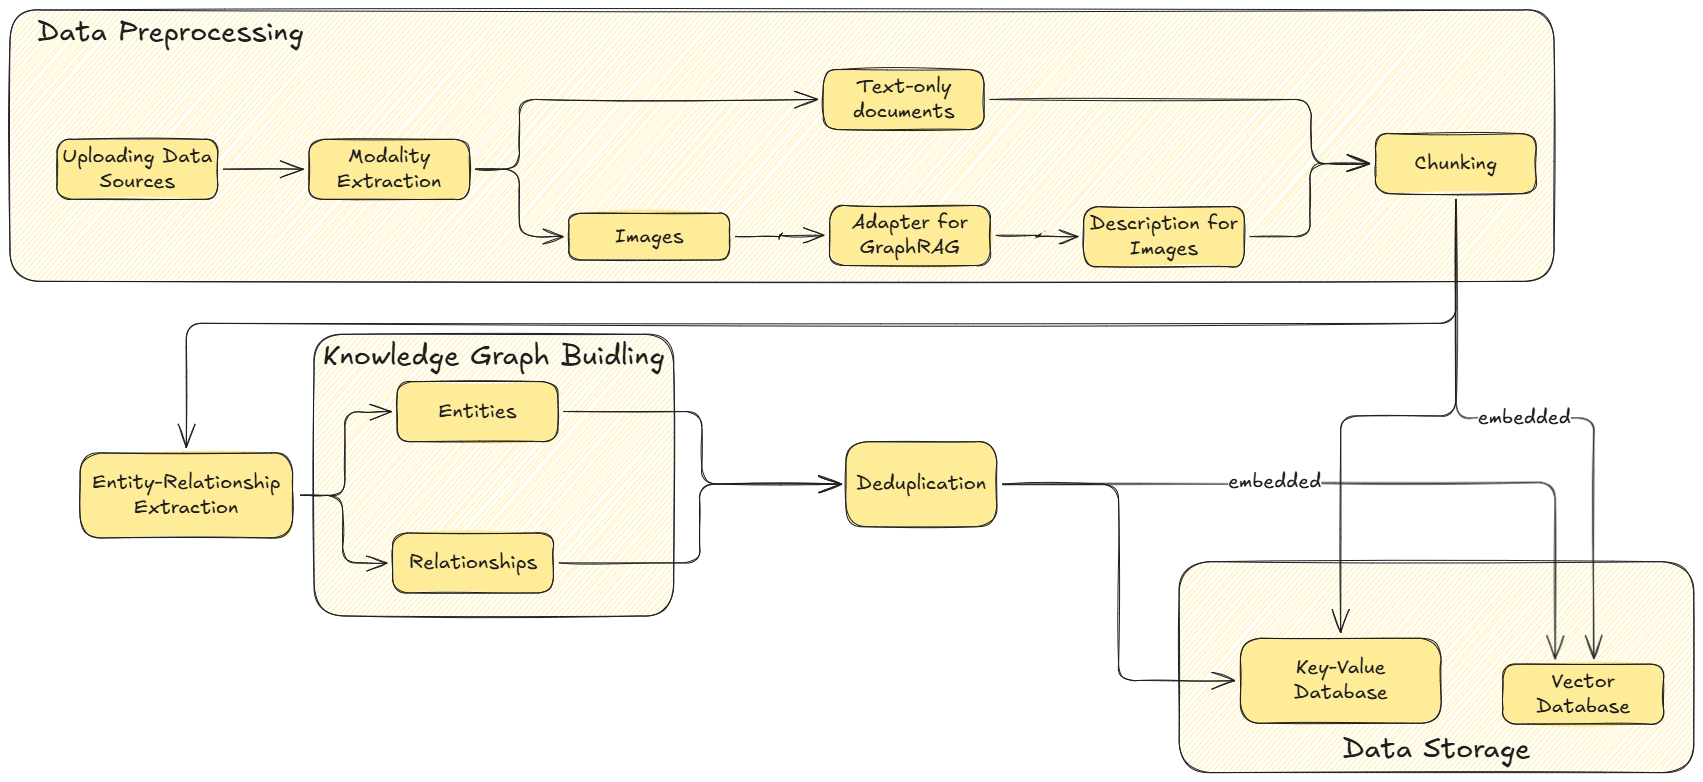
\includegraphics[width=\columnwidth]{figures/RAG_Data_Ingestion_Flow.png}
    \caption{Overview of data ingestion process}
    \label{fig:data-ingestion}
    \end{figure}
    \item Retrieval phase: As illustrated in Fig.~\ref{fig:retrieval}, when a user query is given, the retrieval process operates simultaneously in three modes. In the Naive mode, vector similarity is computed directly between the embedded user query and embedded data chunks to retrieve the most similar chunks. In the Local and Global modes, embeddings of entities and relationships are compared with the embedded user query, after which the most similar entities and relationships are mapped to their corresponding data chunks. Finally, data chunks retrieved from all three modes are aggregated and reranked based on their relevance to the query before being returned.
    \begin{figure}[htbp]
    \centering
    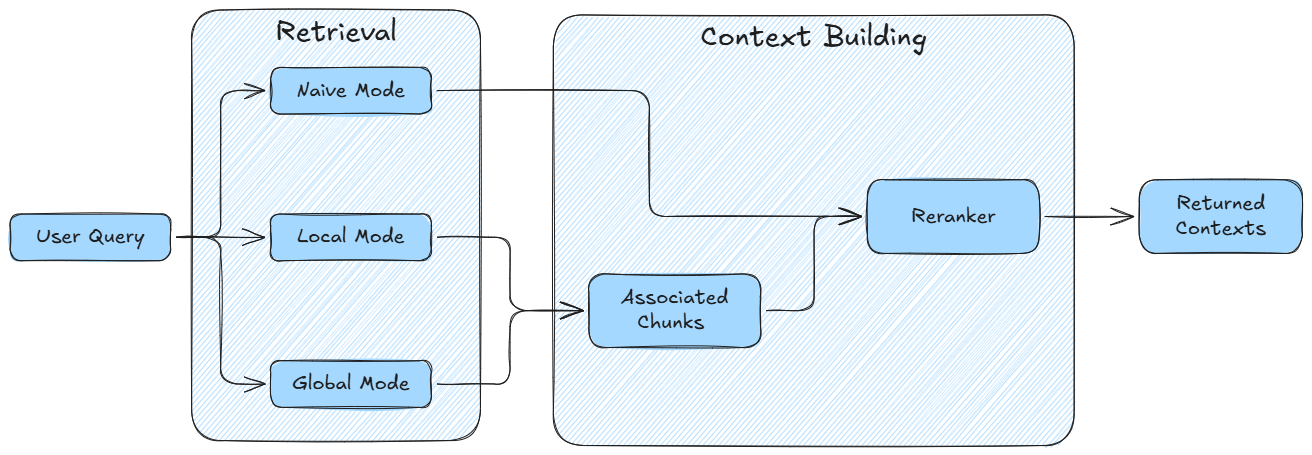
\includegraphics[width=\columnwidth]{figures/RAG_Retrieval_Flow.png}
    \caption{Overview of retrieval process}
    \label{fig:retrieval}
    \end{figure}
\end{enumerate}

\subsubsection{Fine-tuning Pipeline}
\label{sec:finetuning-pipeline}

\paragraph{Overview Fine-tuning}
Fine-tuning adapts a pre-trained large language model to a specific task or domain using supervised data. In this work, we employ instruction fine-tuning, training the model on our generated question–answer dataset. The objective is to teach the model to perform clinical diagnosis following the format proposed in the MedCaseReasoning paper, which includes both the final diagnosis and the corresponding reasoning. Through this process, we aim to improve diagnostic accuracy while producing more coherent and plausible reasoning, which improves the interpretability in sensitive medical contexts. Fine-tuning is implemented using NVIDIA NeMo, a framework optimized for efficient GPU-based training.

\paragraph{Fine-tuning Pipeline}
As illustrated in Fig.~\ref{fig:fine-tune-pipeline}, the fine-tuning pipeline in NeMo generally has five steps.

\begin{enumerate}[label=\roman*.]
    \item Step 1: We take in the benchmark dataset as a csv file.
    \item Step 2: We convert the dataset into NeMo-compatible formats, particularly WebDataset (WDS) shards and ingest it through NeMo’s data loader.
    \item Step 3: We set training configuration and select model components (e.g., attention layers) for LoRA fine-tuning according to the provider's recipe.
    \item Step 4: The fine-tuning process is executed using NeMo’s trainer module and monitored using Weight and Biases (Wandb).
    \item After training, the learned LoRA adapters or fine-tuned checkpoints are exported. During inference later, we can serve the resulting model using vLLM.
\end{enumerate}

\begin{figure}[htbp]
\centering
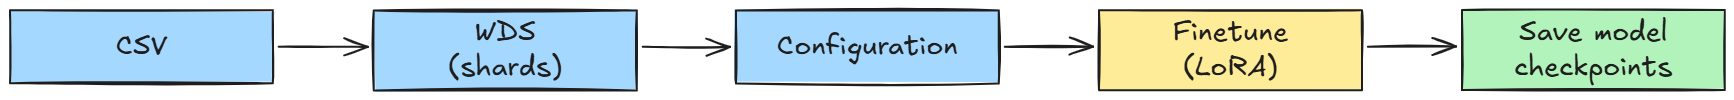
\includegraphics[width=\columnwidth]{figures/Finetune_Pipeline.png}
\caption{Overview of fine-tuning pipeline}
\label{fig:fine-tune-pipeline}
\end{figure}

\paragraph{Fine-tuning Configuration}
We fine-tune the Gemma-4B-IT model using a parameter-efficient approach based on Low-Rank Adaptation (LoRA), optimized with the Adam optimizer. The LoRA configuration uses a rank of $r=4$ and a scaling factor of $\alpha=16$. Training is performed for a maximum of 1,000 steps with early stopping applied using a patience of 10 steps. The learning rate is set to $1\times10^{-5}$, with a weight decay of 0.01.

The dataset consists of 109 cases and is split into training and validation sets using an 9:1 ratio. All experiments are conducted on a single NVIDIA RTX 4090 GPU.

\subsubsection{Hybrid Combination Approach and User Interface}
\label{sec:hybrid-approach}

\paragraph{Combination Overview}

To leverage the strengths of both methods, we integrate them into a unified pipeline using LangGraph. As illustrated in Fig.~\ref{fig:combined-pipeline}, which is visualized through the built-in LangGraph CLI interface, the overall workflow consists of three main steps: case extraction, model calling, and result export. Within the model invocation step, a conditional mechanism allows users to select among four operating modes: a baseline model only, a model augmented with \ac{RAG}, a fine-tuned model, and a model enhanced with both \ac{RAG} and fine-tuning.

During inference, the user provides a clinical question along with associated images, either as local file paths or in Base64 format. The \ac{RAG} system first retrieves relevant contextual information based on the question and then concatenates the question, the images (with local files loaded and encoded into Base64), and the retrieved context into a single model input. The pipeline produces a concise output that directly answers the question, such as a diagnosis or symptom, followed by the corresponding reasoning. The system prompt and the concatenated prompt format used during inference are provided in the Appendix.

\begin{figure}[htbp]
\centering
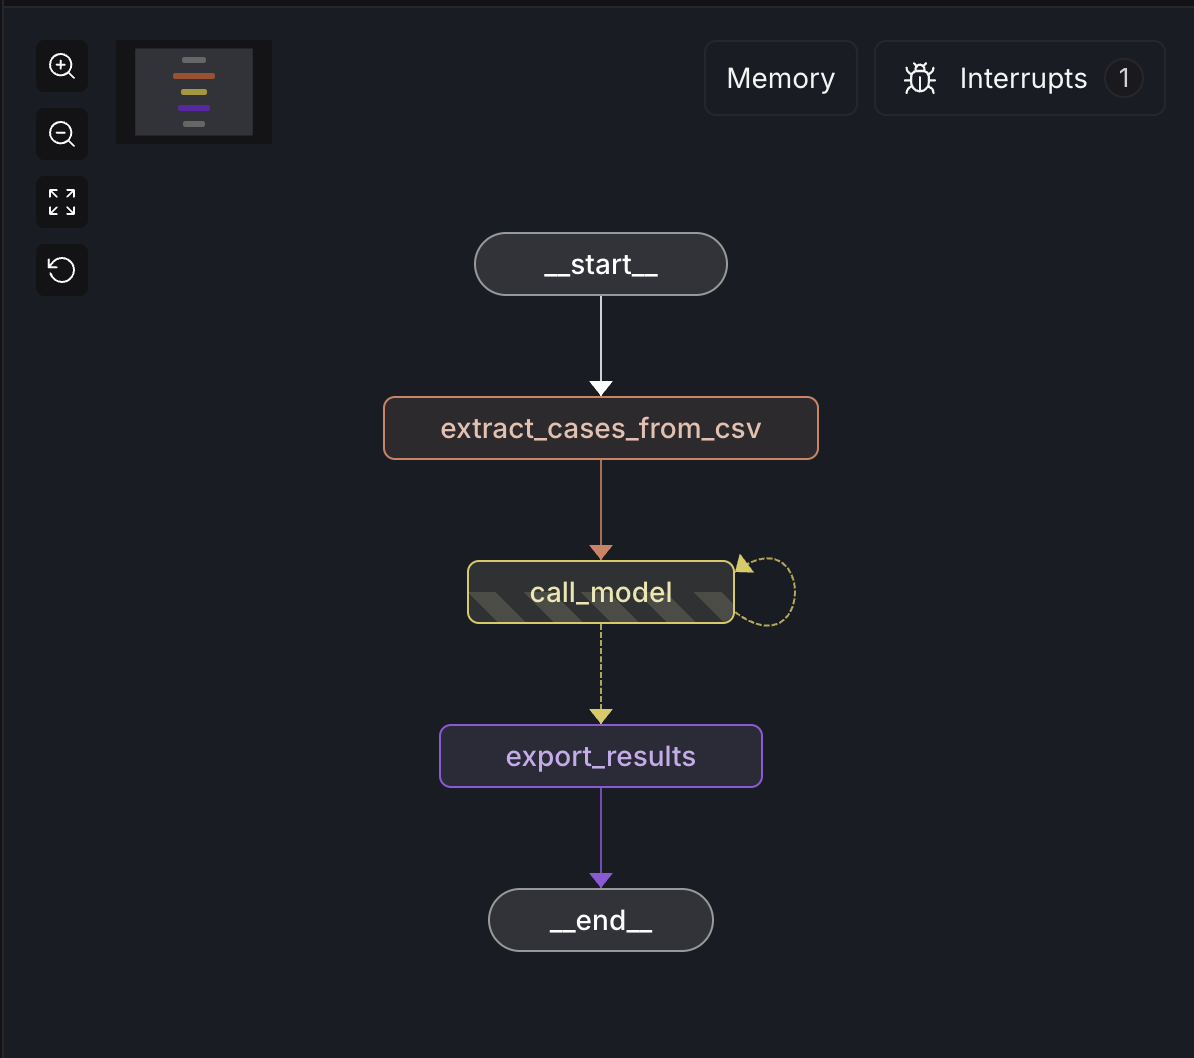
\includegraphics[width=\columnwidth]{figures/Combined_Flow.png}
\caption{Overview of combined pipeline}
\label{fig:combined-pipeline}
\end{figure}

\paragraph{User Interface}
To simulate real usage and bring the application closer to its intended end users, such as patients and clinicians, we developed an interface based on the LangGraph CLI that enables real-time chat with support for image attachments. Although the diagnostic process is currently limited to single-turn interactions, the interface abstracts away technical details and allows users to focus on the system’s functionality. A demonstration conversation between a human user and the AI system is shown in Fig.~\ref{fig:combined-ui}. The AI first presents a concise answer, followed by the corresponding reasoning.
\begin{figure}[htbp]
\centering
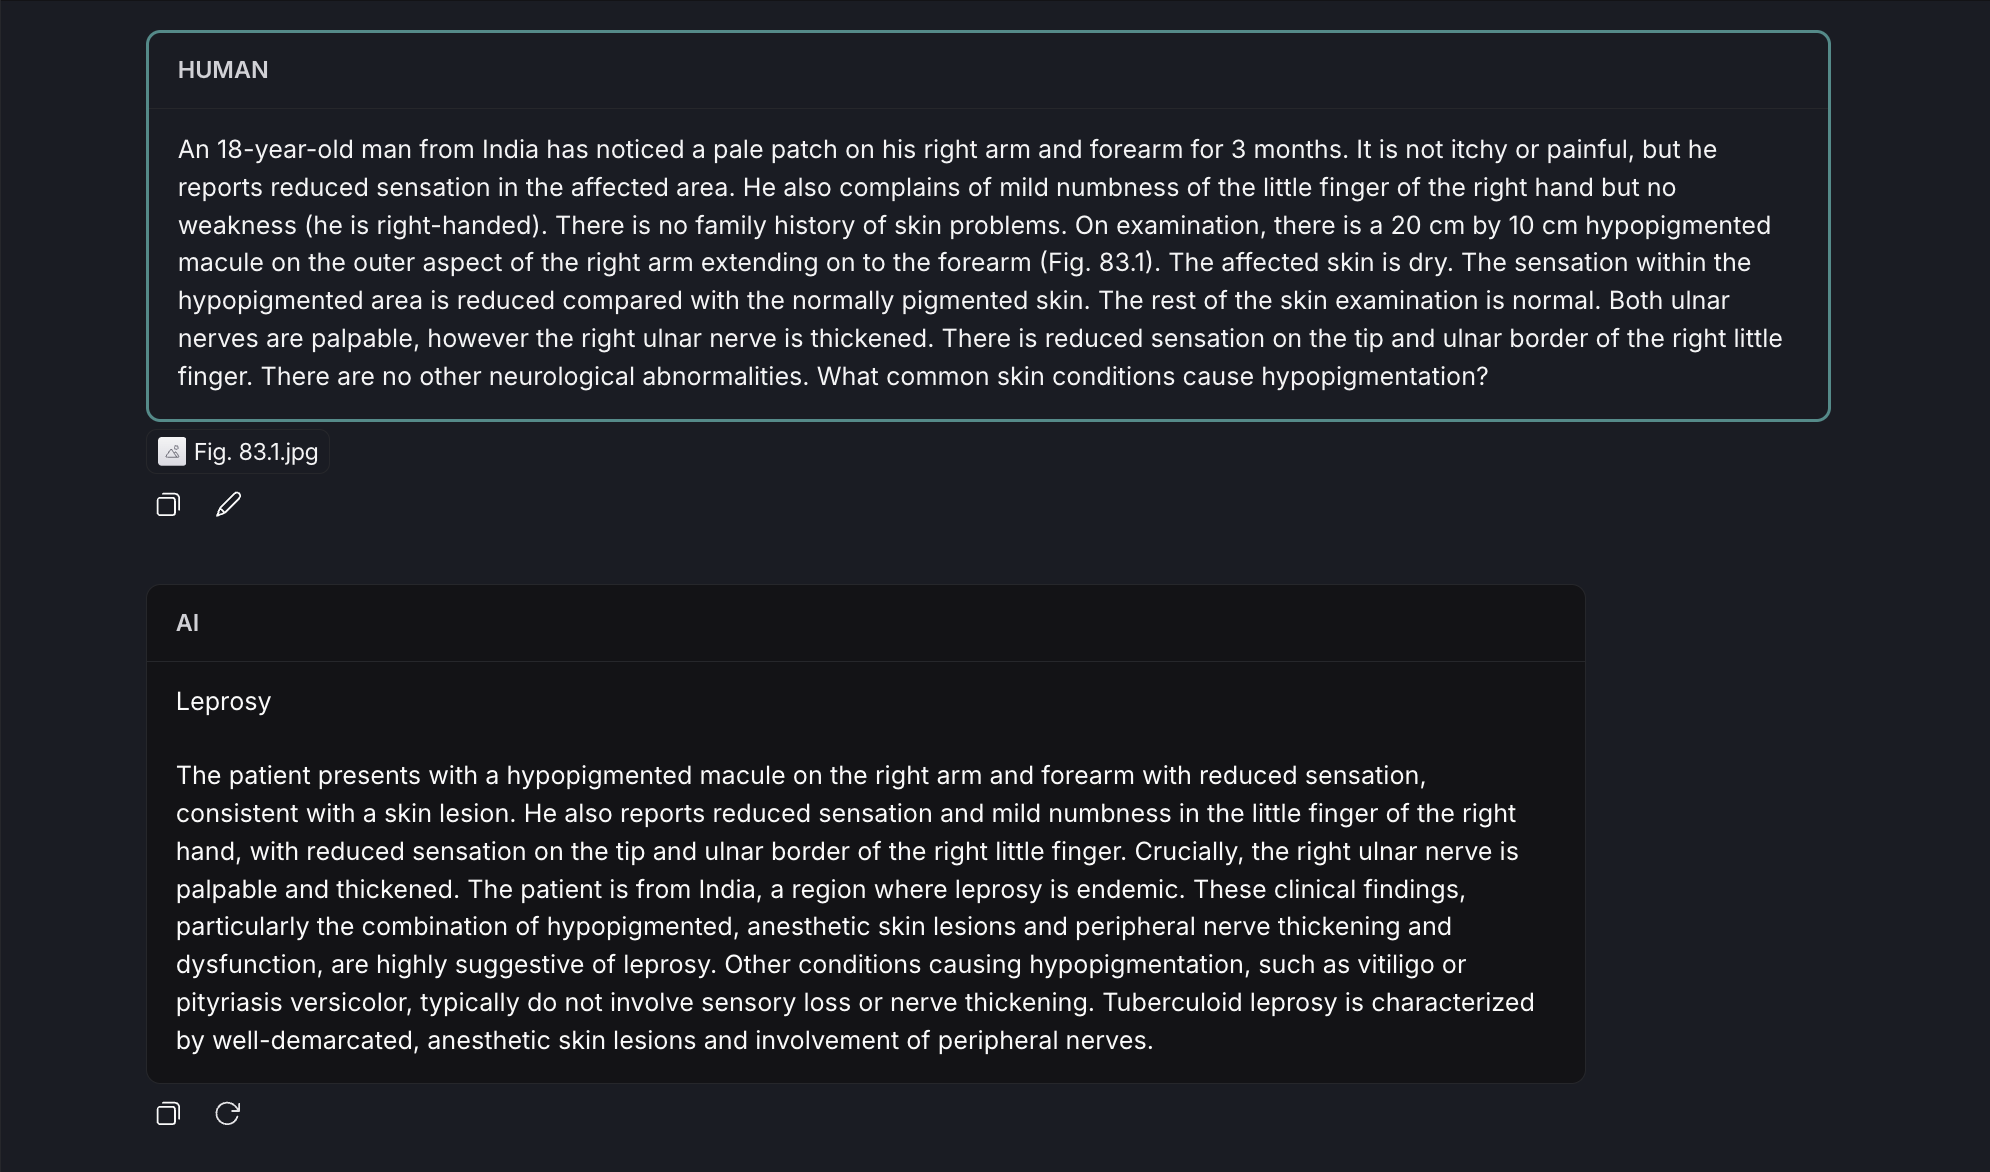
\includegraphics[width=\columnwidth]{figures/Combined_UI.png}
\caption{Overview of user interface}
\label{fig:combined-ui}
\end{figure}